%%%%%%%%%%%%%%%%%%%%%%%%%%%%%%%%%%%%%%%%%%%%%%%%%%%%%%%%%%%%%%%%%%%%%%%%%%
% Copyright (c) 2011, ETH Zurich.
% All rights reserved.
%
% This file is distributed under the terms in the attached LICENSE file.
% If you do not find this file, copies can be found by writing to:
% ETH Zurich D-INFK, Universitaetstr. 6, CH-8092 Zurich. Attn: Systems Group.
%%%%%%%%%%%%%%%%%%%%%%%%%%%%%%%%%%%%%%%%%%%%%%%%%%%%%%%%%%%%%%%%%%%%%%%%%%

\documentclass[a4paper,twoside]{report} % for a report (default)

\usepackage{bftn,color} % You need this
\usepackage{subfig}
\usepackage{listings}
\usepackage{verbatim}

\title{Barrelfish Architecture Overview}   % title of report
\author{Team Barrelfish}	% author
\tnnumber{000}  % give the number of the tech report
\tnkey{Barrelfish Overview} % Short title, will appear in footer

% \date{Month Year} % Not needed - will be taken from version history

%% \newcommand{\note}[1]{}
\newcommand{\note}[1]{[\textcolor{red}{\textit{#1}}]}

\begin{document}
\maketitle

%
% Include version history first
%
\begin{versionhistory}
\vhEntry{1.0}{24.06.2010}{ikuz, amarp}{Initial version}
\vhEntry{2.0}{04.12.2013}{troscoe,shindep}{Extensively updated}
\end{versionhistory}

% \intro{Abstract}		% Insert abstract here
% \intro{Acknowledgements}	% Uncomment (if needed) for acknowledgements
\tableofcontents		% Uncomment (if needed) for final draft
% \listoffigures		% Uncomment (if needed) for final draft
% \listoftables			% Uncomment (if needed) for final draft



%%%%%%%%%%%%%%%%%%%%%%%%%%%%%%%%%%%%%%%%%%%%%%%%%%%%%%%%%%%%%%%%%%%%%%%%%%%%%%%%
\chapter{Barrelfish Architecture Overview}

This document is intended as an introduction to Barrelfish. 
It presents a high level overview of the architecture of the Barrelfish
Operating System, together with the most important concepts used
inside the OS at various levels.  

It does not provide a ``getting started'' guide to running Barrelfish
on a PC, or in an emulation enviroment like Qemu or GEM5 - this is
provided in other documentation.  

\section{High level overview}\label{sec:overview}

Barrelfish is ``multikernel'' operating
system~\cite{barrelfish:sosp09}: it consists of a small kernel running on each core (one kernel per core), and while rest of the
OS is structured as a distributed system of single-core processes atop
these kernels.  Kernels share no memory, even on a machine with
cache-coherent shared RAM, and the rest of the OS does not use shared
memory except for transferring messages and data between cores, and
booting other cores.  Applications can use multiple cores and share
address spaces (and therefore cache-coherent shared memory) between
cores, but this facility is provided by user-space runtime libraries. 

Figure~\ref{fig:os-arch} shows an overview of the components of the OS.  Each
core runs a kernel which is called a "CPU driver". The CPU driver maintains
capabilities, executes syscalls on capabilities, schedules dispatchers, and
processes interrupts, pagefaults, traps, and exceptions.

The kernel schedules and runs "Dispatchers". Dispatchers are an
implementation of a form of scheduler
activations~\cite{Anderson:1991:SAE:121132.121151} (the term is
borrowed from K42~\cite{k42:scheduling}), thus each dispatcher can run
and schedule its own threads.  Multiple dispatchers can be combined
into a domain. Typically this is used to combine related dispatchers
running on different cores. Often dispatchers in a domain share (all
or part of) their vspace. Unless dispatchers in a domain run on the
same core (which is possible, but rare) they cannot share a cspace
(since cspaces are core specific).

Typically we refer to user level processes (or services or servers) as "user
domains". Often these consist of a single dispatcher running on a single core.

\begin{figure}[hbt]
 \begin{center}
 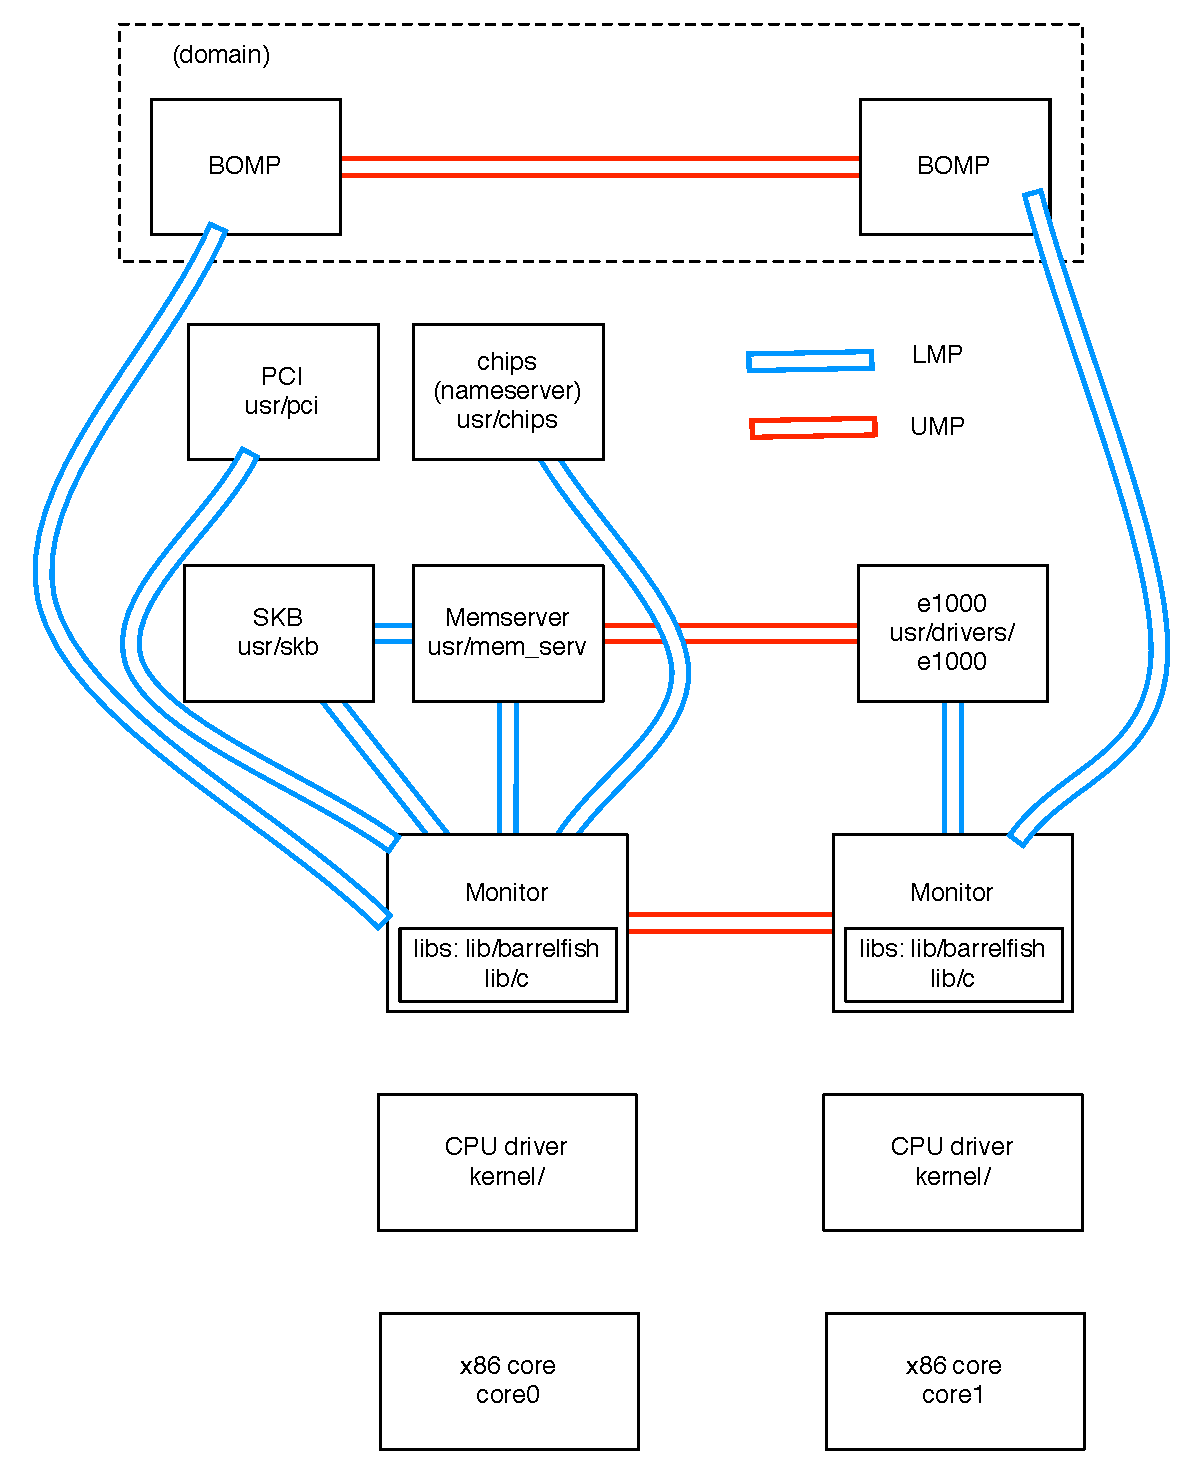
\includegraphics[width=0.5\columnwidth]{os-arch.pdf}
 \end{center}
 \caption{High level overview of the Barrelfish OS architecture}\label{fig:os-arch}
\end{figure}

\section{CPU drivers}

The kernel which runs on a given core in a Barrelfish machine is
called a \emph{CPU driver}.  Each core runs a separate instance of the
CPU driver, and there is no reason why these drivers have to be the
same code.  

In a heterogeneous Barrelfish system, CPU drivers will be different
for each architecture.  However, even on a homogeneous machine, CPU
drivers for different cores can be specialized for some purposes (for
example, some might suppose virtualization extensions, while others
might be optimized for running a single application).  

CPU drivers are single-threaded and non-preemptible.
They run with interrupts disabled on their core, and share no state
with other cores.  CPU drivers can be thought of as serially executing
exception handlers for events such as interrupts, faults, and system
calls from user-space tasks.  Each such handler executes in bounded time
and runs to completion.  If there are no such handlers to execute, the
CPU driver executes a user-space task. 

The functions of a CPU driver are to provide:
\begin{itemize}
\item Scheduling of different user-space \textit{dispatchers} on the
  local core.
\item Core-local communication of short messages between dispatchers
  using a variant of Lightweight RPC~\cite{lrpc:tocs90} or L4
  RPC~\cite{Liedtke:1993:IIK:168619.168633}. 
\item Secure access to the core hardware, MMU, APIC, etc.
\item Local access control to kernel objects and physical memory by
  means of capabilities
\end{itemize}

CPU drivers do not provide kernel threads, for two reasons.  Firstly,
the abstraction of the processor provided to user space programs is a
dispatcher, rather than a thread.  Secondly, since the kernel is
single-threaded and non-preemptible, it uses only a single, statically
allocated stack for all operations. After executing a single exception
handler, the contents of this stack are discarded and reset. 

CPU drivers schedule dispatchers.  The scheduling algorithm employed
by a given CPU driver binary is configurable at compile time, and two
are currently implemented:
\begin{itemize}
\item A simple round-robin scheduler.  This is primarily used for
  debugging purposes, since its behavior is easy to understand.
\item A rate-based scheduler implementing a version of the RBED
  algorithm~\cite{Brandt:2003:DIS:956418.956606}. This is the
  preferred per-core scheduler for Barrelfish, and provides efficient
  scheduling of tasks with a variety of hard and soft realtime jobs
  with good support for best-effort processes as well. 
\end{itemize}

\section{Dispatchers}

The dispatcher is the unit of kernel scheduling, and on a single core
roughly corresponds to the concept of process in Unix.  

A dispatcher can be thought of as the local component of an
application (often called a \textit{domain} in Barrelfish) on a
particular core.  An application which spans multiple cores (for
example, an OpenMP program) has a dispatcher on each core that it
might potentially execute on.  

Operating system tasks in Barrelfish are always single-core by design,
and therefore have only one dispatcher.  Applications, however,
frequently have more, one on each core. 

Dispatchers do not migrate between cores. 

When a CPU driver decides to run a dispatcher as a result of a
scheduling decision, it
\emph{upcalls}~\cite{Clark:1985:SSU:323647.323645} into the dispatcher
as an exit from kernel mode in the manner described below.  The
user-level code associated with the dispatcher then executes
user-space thread scheduling, as well as handling other events (such
as a page fault signal from the kernel or the arrival of an
inter-domain message). 

\begin{figure}[hbt]
 \begin{center}
 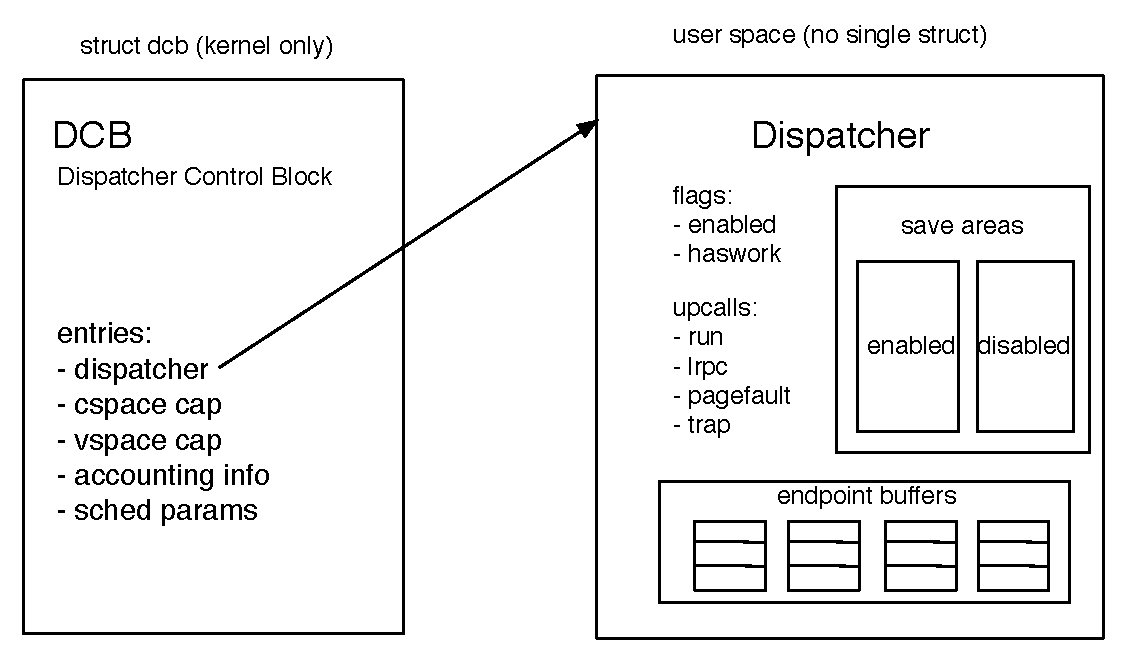
\includegraphics[width=0.5\columnwidth]{dcb.pdf}
 \end{center}
 \caption{Dispatcher Control Block}\label{fig:dcb}
\end{figure}

The kernel maintains a DCB (dispatcher control block) for each dispatcher
(Figure~\ref{fig:dcb}). The DCB contains entries that define the dispatcher's
cspace (capability tables), vspace (page tables), some scheduling parameters,
and a pointer to a user space dispatcher structure (actually it consists of
several structs). This struct manages the scheduling of the dispatcher's
threads.

The dispatcher can be in one of two modes: enabled and disabled. It is in
enabled mode when running user thread code. It is in disabled mode when running
dispatcher code (e.g., when managing TCBs, run queues, etc.). The dispatcher
defines a number of upcall entry points that are invoked by the kernel when it
schedules the dispatcher.

The main upcall is \texttt{run()}.  When the kernel decides to schedule a
dispatcher, it brings in the base page table pointed to by the vspace
capability, and calls the dispatcher's \texttt{run()} upcall.  The dispatcher
must decide which thread it wants to run, restore the thread's state, and then
run it. Note that when \texttt{run()} is invoked the dispatcher first runs in
disabled mode until the thread actually starts executing at which point the
dispatcher switches to enabled mode.

When a dispatcher running in enabled mode is preempted, the kernel saves all
register state to a save area (labelled "enabled"). When the dispatcher is next
restarted it can restore this register state and run the preempted thread, or it
can decide to schedule another thread, in which case it must first save the
saved registers to a TCB.  

When the kernel preempts a dispatcher running in disabled state, it stores the
register state in a save area labelled "disabled". When the kernel schedules a
dispatcher that is in disabled state, it does not invoke \texttt{run()}. Instead
it restores the registers stored in the disabled save area. This causes the
dispatcher to resume execution from where it was preempted.

\section{Runtime libraries}

The basic runtime of any Barrelfish program is two libraries: a
standard C library (currently a version of
\texttt{newlib}~\cite{newlib}), and \texttt{libbarrelfish}.  In
practice the two libraries are inter-dependent, though there is an
ongoing effort to minimize truly cyclic dependencies.  The principal
cycles involve \texttt{malloc()} and communication with the memory
server. 

The barrelfish library implements the following functionality:
\begin{itemize}
\item User-level thread scheduling, based on the upcall model of the
  dispatcher.
\item Physical memory management by communication with the memory
  server. 
\item Capability management (maintaining the domain's cspace),
  including allocating new CNodes where necessary. 
\item Construction of virtual address spaces using capability
  invocations.
\item User-level page fault handling.
\item Communications using message channels, including blocking and
  nonblocking calls on channels, and the implementation of
  \texttt{waitset}s (analogous to Unix \texttt{select()} and
  \texttt{epoll()}). 
\end{itemize}

\section{Capabilities}

Barrelfish uses a single model of
\emph{capabilities}~\cite{hank:capabilities} to control access to all
physical memory, kernel objects, communication end-points, and other
miscellaneous access rights. 

The Barrelfish capability model is similar to the seL4
model~\cite{sel4:iies08}, with a considerably larger type system and
extensions for distributed capability management between cores. 

Kernel objects are referenced by partitioned capabilities. The actual
capability can only be directly accessed and manipulated by the
kernel, while user level only has access to capability references
(\texttt{struct capref}), which are addresses in a cspace. User level
can only manipulate capabilities using kernel system calls (to which
it passes capability references). In processing a system call the 
kernel looks up the capability reference in the appropriate cspace to find the
actual capability; this process is similar to the translation of a virtual
address to a physical address (Figure~\ref{fig:cap_translation}). A capability
reference can be used to get \texttt{caddr\_t} and \texttt{valid bits} which are
used in system calls (see \texttt{include/barrelfish/caddr.h}).  Valid bits are
used when the user wants to access cnode type capabilities (else, the
translation process would continue by looking at entries in the cnode).
 
\begin{figure}
  \centering
  \subfloat[capref to capability translation.]{\label{fig:cap_translation}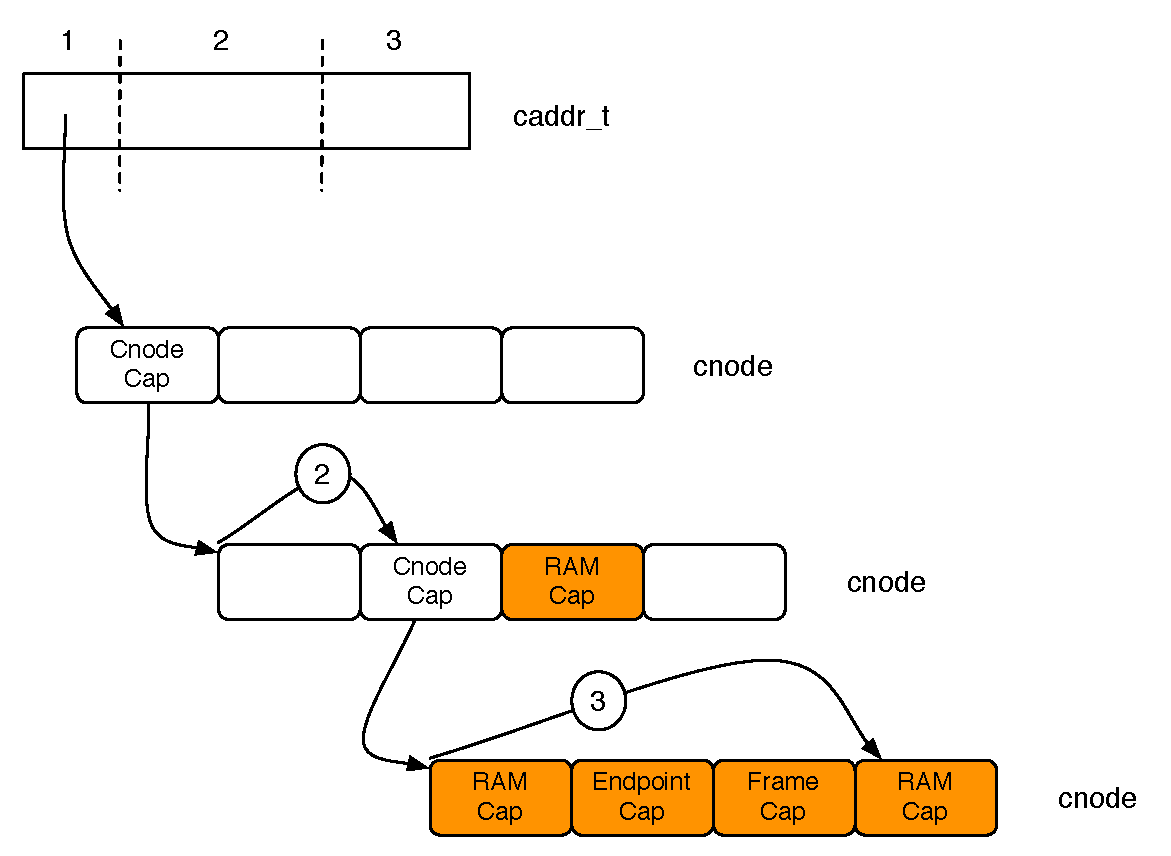
\includegraphics[width=0.4\textwidth]{cap_translation.pdf}}
  \quad
  \subfloat[Capability Hierarchy]{\label{fig:cap_hierarchy}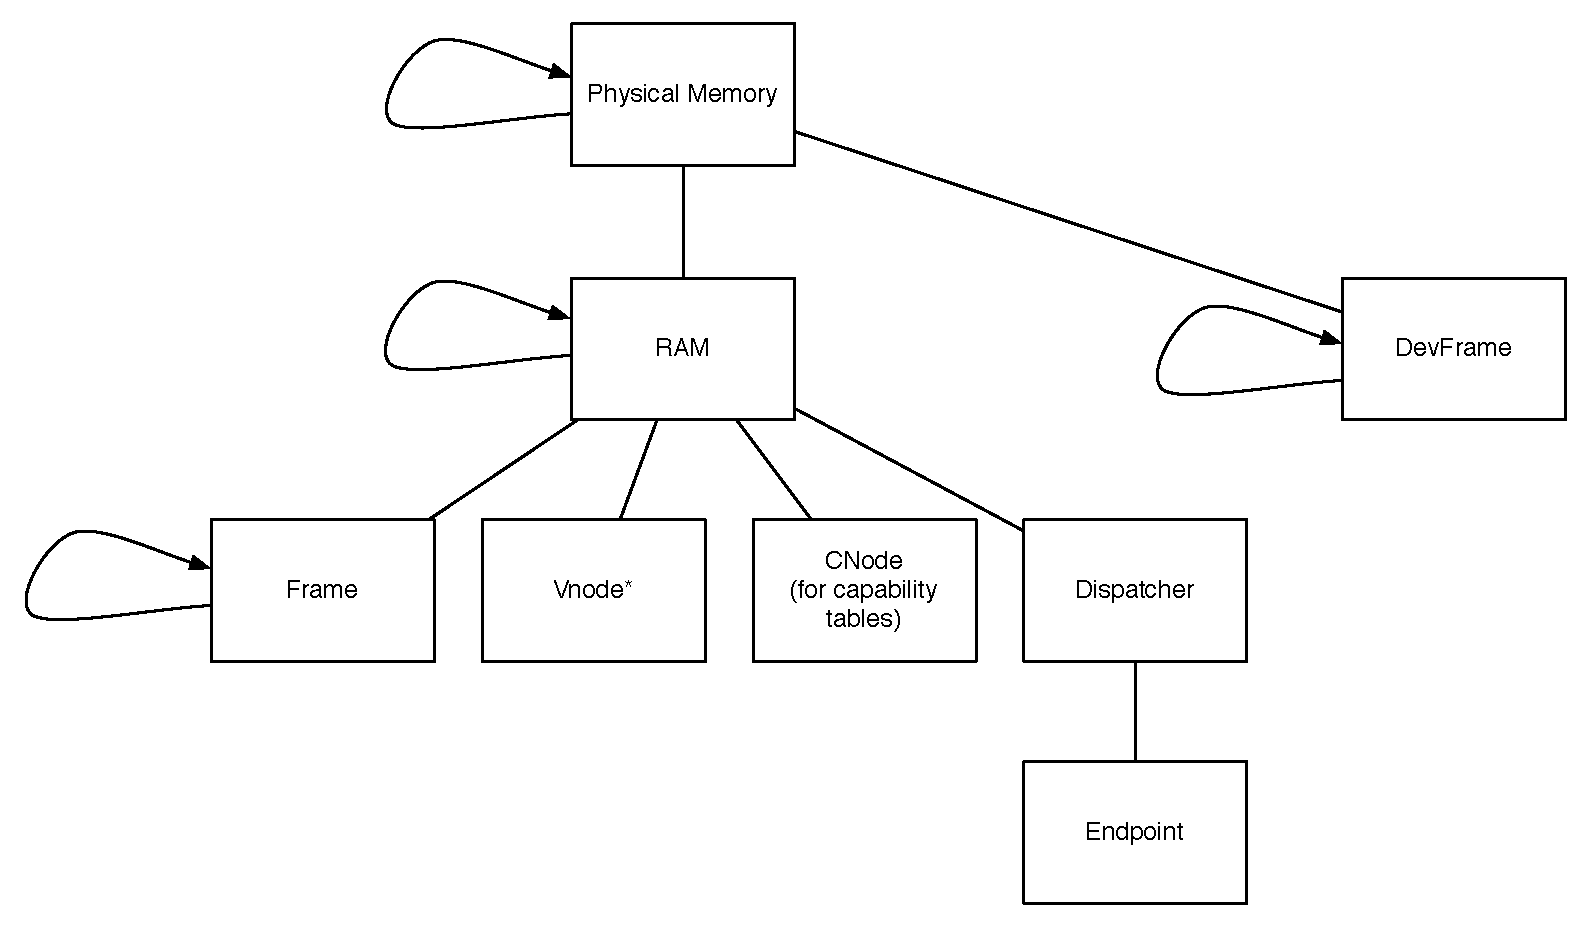
\includegraphics[width=0.5\textwidth]{cap_heirarchy.pdf}}
  \caption{Capabilities}
  \label{fig:caps}
\end{figure}

A Dispatcher only has access to the capability references in its cspace. As in
seL4, capabilities are typed, and there is a strictly defined derivation
hierarchy (e.g. Figure~\ref{fig:cap_hierarchy}).  The type system for
capabilities is defined using a domain-specific language called
Hamlet. 

\section{Physical Memory}

All regions of physical address space are referred to by means of
capabilities.  At present, a memory capability refers to a
naturally-aligned, power-of-two-sized area of at least a physical page
in size, though this restriction is likely to go away in the future. 

A memory capability can be split into smaller capabilities, and this
basic mechanism is used for low-level physical memory allocation. 

Memory capabilities are \emph{typed}, and each region type supports a
limited set of operations.  Initially, memory consists of untyped RAM
and \emph{device frames}, which are used to refer to memory-mapped I/O
regions. 

RAM capabilities can be retyped into other types; the precise number
is defined in the Hamlet language in a file currently located in
\texttt{/capabilities/caps.hl}.  Some of the more common types of
memory capability are:
\begin{itemize}
\item \emph{Frame} capabilities are RAM capabilities which can be
  mapped into a user's virtual address space.
\item \emph{CNode} capabilities are used to hold the bit
  representation of other capabilities, and construct a domain's
  cspace.  CNodes can never be mapped as writeable virtual memory,
  since this would remove the security of the capability system by
  allowing an application to forge a capability.
\item \emph{Dispatcher} capabilities hold dispatcher control blocks.
\item \emph{Page table} capabilities refer to memory which holds page
  table pages.  There is a different capability type for each level of
  each type of MMU architecture.
\end{itemize}

\section{Virtual Memory}

Barrelfish applications are
\emph{self-paging}~\cite{Hand:1999:SNO:296806.296812}: they securely
construct and maintain their own page tables, and page faults are
reflected back to the application by means of an upcall. 

An application constructs its own virtual address space (generally
abbreviated to \emph{vspace}) using the capability system.  It
acquires RAM from a memory allocator in the form of RAM capabilities,
and then retypes these to frames and page tables.  

To take a 32-bit x86 machine without Physical Address Extensions (PAE)
as a simple example, to map a frame into its vspace an application
invokes the capability refering to a Page Table page using a system
call.  The arguments to this capability invocation are (1) a
capability for a 4kB frame, (2) a slot number (from 0 to 1023), and
(3) a set of mapping flags.  This will cause the kernel to insert a
Page Table Entry (PTE) with the appropriate flags into the
corresponding slot in the Page Table.

Note that, while the user determines exactly what mapping is entered
in the page table, the process is secure: the user cannot map a frame
that they do not already hold a capability for, that capability must
refer to a frame (and not some other type of memory, such as a
dispatcher control block or CNode), and they must also hold a
capability for the page table itself. 

Similarly, in this example, for the Page Table page to be useful it
must itself be referenced from a Page Directory.  To ensure this, the
user program must perform a similar invocation on the Page Directory
capability, passing the slot number, flags, and the capability to the
Page Table page.  As before, the capability type system allows neither
the construction of an invalid page table for any architecture, nor
the mapping of any page that the user has no authorization for. 

This model also has the additional feature that any core can construct
a valid page table for any other core, even if the cores have
different MMU architectures.  An x86\_64 core can construct a valid
and secure ARMv7 virtual address space, and pass a capability for the
L1 Page Table of this vspace to an ARMv7 core for installation. 

Furthermore, since the application is responsible for constructing
page tables and allocating physical memory itself, it can handle page
faults by changing its own mappings, potentially paging data to and
from stable storage in the process. 

Naturally, this pushes significant complexity into the application.
Paging functionaly is generally hidden in the runtime
\texttt{libbarrelfish} library, though is available for direct
manipulation for non-common use cases. 

\section{Inter-domain communication}

Barrelfish provides a uniform interface for passing messages between
domains, which handles message formating and marshalling, name
lookup, and end-point binding.  

This interface is \emph{channel-based}: for two domains to
communicate, they must first establish a channel (which may involve
agreeing on some shared state).  Messages are thereafter sent on this
channel.  The process of establishing channel state is known as
\emph{binding}.

A channel is typed, and the type determines the kinds of messages that
can be sent on it.  As with many RPC systems, channel types are
defined using an \emph{interface definition language}, which in
Barrelfish is known as Flounder.    Flounder interface types are
generally found in the \texttt{/if} directory in the Barrelfish tree.
Messages can pass both simple data types and, optionally,
capabilities. 

To establish a communications channel, a domain typically has to
acquire an \emph{interface reference} from somewhere, which identifies
the remote endpoint it will try to connect to.  In the common case,
this is obtained from the System Knowledge Base, acting as a name
server. After having bound an interface reference, the result is a
local stub object at either end of the channel which can be called to
send a message, and also implements dispatch of received messages. 

In turn, an interface reference is created by a server creating a
service (analogous to a listening socket) and registering this with a
name service. 

There are a variety of underlying implementations of message passing
in Barrelfish, known as \emph{Message Transports}.  Each one is highly
optimized for a particular hardware scenario.  In general, the binding
process automatically selects the appropriate transport for a channel,
though this process can also be overwritten. 

A message transport itself consists of several components:
\begin{enumerate}
\item An \emph{interconnect driver} or ICD sends small, fixed-size
  units of data between domains.  This is highly optimized: for
  same-core message passing, the LMP (``local message passing'') ICD
  is based on L4's RPC path, while between cache-coherent cores the
  UMP (``user-level message passing'') ICD is similar to
  URPC~\cite{urpc:tocs91} or
  FastForward~\cite{Giacomoni:2008:FEP:1345206.1345215} and transfers
  single cache lines without involving the kernel.  Other ICDs exist
  for specialized messaging hardware, and/or network communication.

  ICDs do \emph{not} export a standard interface; each one is
  different. 
\item \emph{Stubs} generated by Flounder from an interface
  specification provide the uniform interface to clients and servers,
  and perform the abstraction of ICDs, as well as handling message
  fragmentation and reassembly in the cases where an application
  message is larger than the unit transferred by the ICD.  Since
  different ICDs do not export the same interface, there is a
  different Flounder code generator for each ICD type, enabling
  cross-layer optimizations not possible otherwise. 
\item Finally, some stubs can also invoke separate \emph{Notification
  Drivers}, which provide a synchronous signal to the receiving domain
  in cases where the transfer of the message payload itself does not.
  For example, UMP messages have to be polled by the reciever by
  default, but on some architectures an additional notification driver
  can be invoked by the stub to cause an inter-processor interrupt
  (IPI) after some time if the other end of the channel appears to be
  asleep. 
\end{enumerate}

In addition, stubs can also handle other areas of complexity resulting
from the optimized nature of interconnect drivers.  For example,
capabilities cannot be sent directly over a UMP channel, since their
bit representations cannot be safely made available to user-space
applications.  Instead, the stubs for UMP transport send capabilities
over a separate, secure channel via the Monitors on the sending and
receiving cores, which are themselves contacted using LMP (which can
transfer capabilities) by the sending and receiving domains.  

In this way, transfer of pure data over message transports can be
extremely fast, at the cost of extra delay when transferring
capabilities. 

\section{System Knowledge Base}

Barrelfish includes a system service called the System Knowledge Base,
which is used to store, query, unify, and compute on a variety of data
about the current running state of the system.  The SKB is widely used
in Barrelfish; examples are:

\begin{itemize}
\item The Octopus lock manager and pub/sub system is built as an
  extension to the SKB (with a somewhat different interface
  language). 
\item Devices are discovered and entered into the SKB, and the SKB
  contains rules to determine the appropriate driver for each device.
  This forms device management (see below).
\item The PCI driver uses constraint solving in the SKB to correctly
  configure PCI devices and bridges.  The SKB contains a list of known
  PCI quirks, bugs, and special cases that have to taken in to account
  when allocating BAR values for address ranges.  Interrupt routing is
  also performed in the SKB.
\item The SKB functions as a general-purpose name server / interface
  trader for the rest of the OS.
\item The results of online hardware profiling are entered into the
  SKB at boottime, and can be used to construct optimal communication
  patterns in the system.
\end{itemize}

The SKB implemention for Intel architectures is currently based on a
port of the eCLiPse constraint logic programming
system~\cite{eclipse}.  This consists of a Prolog interpreter with
constraint solving extensions, and has been extended with a fast
key-value store which can also retain capabilities.  Aside from the
Octopus interface, it is possible to communicate with the SKB by
sending Prolog expressions as messages.

\section{Device drivers}

Device drivers in Barrelfish are implemented as individual dispatchers
or domains.  When they start up, they are supplied with arguments
which include various option variables, together with a set of
capabilities which authorize the driver to access the hardware device.

The capabilities a driver needs are generally:
\begin{enumerate}
\item \emph{Device frame} capabilities for regions of the physical
  address space containing hardware registers; these regions are then
  memory-mapped by the driver domain as part of its initialization
  sequence. 
\item \emph{Interrupt} capabilities, which can be used to direct the
  local CPU driver to deliver particular interrupt vectors to the
  driver domain. 
\item On x86 machines, \emph{I/O capabilities} allow access to regions
  of the I/O port space for the driver. 
\item For message-based device interfaces, such as USB, there may be
  \emph{communication end-point capabilities} which allow messages to
  be sent between the driver domain and the driver for the host
  interface adaptor itself. 
\end{enumerate}

Hardware interrupts are received by a core, demultiplexed if
necessary, and then turned into local inter-domain messages which are
dispatched to the appropriate driver domain.  Each first-level
interrupt handler disables the interrupt as it is raised.  As in L4,
interrupts are renabled by the driver domain sending a reply message
back to the CPU driver. 

Driver domains themselves then export their functionality to clients
(such as file systems, or network stacks) via further message-passing
interfaces. 

\section{Device management}

Device management in Barrelfish is performed by a combination of
components:
\begin{itemize}
\item The System Knowledge Base is used to store information about all
  discovered hardware in the system.  It also holds the information
  about which driver binaries should be used with which devices, and
  contains rules to determine on which core each device's driver domain
  should run. 
\item Octopus, the Barrelfish locking and pub/sub system built on top
  of the SKB, is used to propagate events corresponding to device
  discovery, hotplug, and driver startup and shutdown. 
\item Kaluga is the Barrelfish device manager, and is responsible to
  starting up driver domains based on information in the SKB and in
  response to events disseminated by Octopus.  It handles passing the
  appropriate authorizations (in the form of device, I/O, and
  interrupt capabilities) to new driver domains. 
\item The driver domains themselves populate the SKB with further
  information about devices. For example, the PCI driver stores
  information about enumerated buses and functions in the SKB, and USB
  Host Adaptor drivers so something similar for enumerated devices.
\end{itemize}

In newer versions of Barrelfish, the same framework is also used for
booting (and suspending or shutting down) cores.  In addition to an
appropriate CPU driver, each core other than the bootstrap core has a
\emph{Boot Driver}, which is responsible for booting the new core and
encapsules the protocol (usually platform-specific) for core startup. 

\section{Monitor}

Each Barrelfish core runs a special process called the \emph{Monitor},
which is responsible for distributed coordination between cores.  All
monitors maintain a network of communication channels among
themselves; any monitor can talk to (and identify) any other monitor.
All dispatchers on a core have a local message-passing channel to
their monitor. 

Monitors are trusted: they can fabricate capabilities. This is because
they are responsible for transferring capabilities between cores, and
so must be able to serialize a capability into bits and reconstruct it
at the other end.  Monitors therefore posess a special capability (the
\emph{Kernel capability}) which allows them to manipulate their local
core's capability database. 

The monitor performs many low-level OS functions which require
inter-core communication (since CPU drivers by design do not
communicate with each other, nor share any memory).  For example: 

\begin{itemize}
\item Monitors route inter-core bind requests for communication
  channels between domains which have not previously communicated
  directly. 
\item They send capabilities along side channels, since regular
  domains on different cores cannot send capabilities directly
  themselves without involving the kernel. 
\item Monitors help with domain startup by supplying dispatchers with
  useful initial capabilities (such as a communication channel back
  to the monitor, and ones to the memory allocator and SKB). 
\item They perform distributed capability revocation, using a form of
  two-phase commit protocol among themselves over the capability
  database. 
\end{itemize}

The monitor contains a distributed implementation of the functionality
found in the lower-levels of a monolithic kernel.  The choice to make
it into a user-space process rather than amalgamating it with the CPU
driver was an engineering decision: it results in lower performance
(many operations which would be a single syscall on Unix require two
full context switches to and from the monitor on Barrelfish).
However, running the monitor as a user-space process means it can be
time-sliced along with other processes, can block when waiting for I/O
(the CPU driver has no blocking operations), can be implemented using
threads, and provides a useful degree of fault isolation (it is quite
hard to crash the CPU driver in Barrelfish, since it performs no
blocking operations and requires no dynamic memory allocation).

\section{Memory Servers}

Memory servers are responsible for serving RAM capabilities to
domains.  A memory server is started with an initial (small) set of
capabilities which list the regions of memory the server is
responsible, and they respond to requests from other domains for RAM
capabilities of different sizes. 

At system startup, there is an initial Memory Server running on the
bootstrap core which is created with a capability to the entire range
of RAM addressable from that core.  However, the use of capabilities
allows this to delegate management of subregions of this space to
other servers.  This is desirable for two reasons:
\begin{itemize}
\item It allows core to have their own memory allocators, greatly
  improving parallelism and scalability of the system. As in other
  systems, Barrelfish's per-core allocators can also steal memory from
  other cores if they become short. 
\item It permits different allocators for different types of memory,
  such as different NUMA nodes, or low-memory accessible to legacy DMA
  devices.
\end{itemize}

Each new dispatcher in Barrelfish is started with a bootstrapped
message channel to its own local memory server. 

\section{Filing system}

Barrelfish at present has no native file system.  However, runtime
libraries do provide a Virtual File System (VFS) interface, and a
number of backends to this exist (and are used in the system),
including:
\begin{itemize}
\item An NFSv3 client.
\item A simple RAM-based file system.
\item Access to the OS multiboot image via the VFS interface.
\item A FAT file system which can be used with the AHCI driver and ATA
  library. 
\end{itemize}

\section{Network stack}

\begin{figure}[hbt]
 \begin{center}
 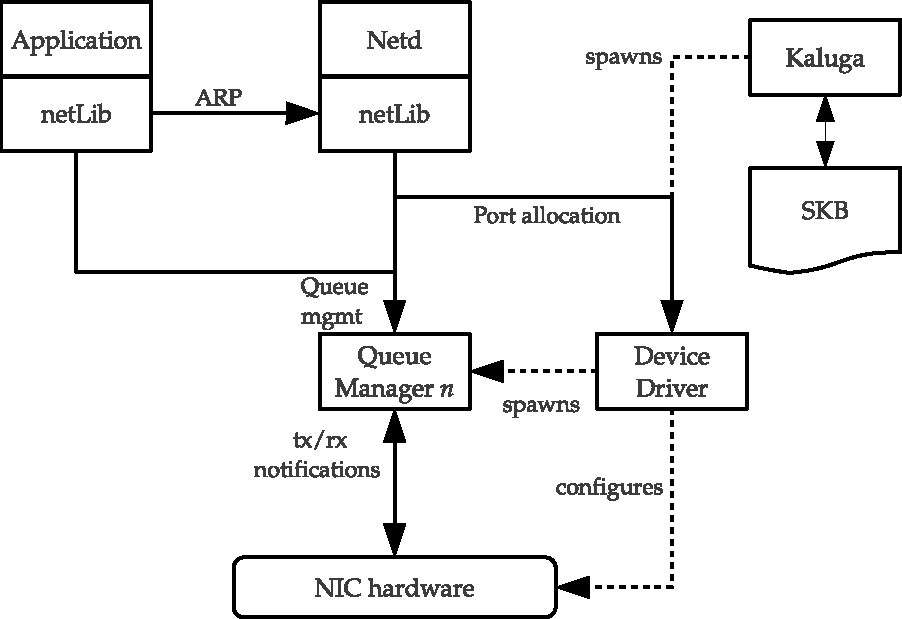
\includegraphics[width=0.7\columnwidth]{net-arch.pdf}
 \end{center}
 \caption{High level overview of the Barrelfish network stack}\label{fig:net-arch}
\end{figure}

At time of writing, the Barrelfish network stack is evolving, but
Figure~\ref{fig:net-arch} shows the high-level structure.  Barrelfish
aims at removing as much OS code from the datapath as possible, and
uses a design inspired by Nemesis~\cite{Black:1997:PIV:648046.745222}
and Exokernel~\cite{Ganger:2002:FFA:505452.505455}. 

Each physical network interface has a driver which is started by the
Kaluga device manager service.  This driver is in turn capable of
initiating a separate \emph{queue manager} for each hardware queue
supported by the network hardware, and configuring the NIC hardware to
demultiplex incoming packets to the appropriate queue.  

Applications run their own network stack on a per-flow basis, either
reading and writing packets directly to and from hardware queues (if
possible), or with the queue manager performing an extra level of
multiplexing on each queue.   The queue manager receives events from
the NIC hardware signalling transmission and reception of packets. 

An additional domain, the network daemon (\texttt{netd}), is
responsible for non-application network traffic (such as ARP requests
and responses, and ICMP packets).  This daemon also handles allocation
of ports from talking to a given network interface. 

%%%%%%%%%%%%%%%%%%%%%%%%%%%%%%%%%%%%%%%%%%%%%%%%%%%%%%%%%%%%%%%%%%%%%%%%%%%%%%%%
\chapter{The Barrelfish source tree}\label{chap:sourcetree}

\newenvironment{dirlist}{%
\let\olditem\item% 
\renewcommand\item[2][]{\olditem \texttt{##1}:\\[0.3\baselineskip]##2}%
\begin{description}}{\end{description}%
}

The Barrelfish source tree is organized as follows:
\begin{dirlist}
\item[capabilities/] Definitions of the capability type system,
  written in the Hamlet language.
\item[devices/] Definitions of hardware devices, written in the
  Mackerel language. 
\item[doc/] \LaTeX Source code for the Barrelfish Technical Notes, including
  this one.
\item[errors/] Definitions of Barrelfish system error codes, written
  in the Fugu language. 
\item[hake/] Source code for the Hake build tool.
\item[if/] Definitions of Barrelfish message-passing interface types,
  written in the Flounder language. 
\item[include/] Barrelfish general header files.
\item[kernel/] Source code for Barrelfish CPU drivers.
\item[kernel/include/] Header files internal to Barrelfish CPU drivers.
\item[lib/] Source code for libraries. 
\item[tools/] Source code for a variety of tools used during the build
  process. 
\item[trace\_definitions/] Constant definitions for use by the
  Barrelfish tracing infrastructure, written in the Pleco language. 
\item[usr/] Source code for Barrelfish binaries. 
\item[usr/drivers/] Source code for Barrelfish device driver binaries.
\end{dirlist}


%%%%%%%%%%%%%%%%%%%%%%%%%%%%%%%%%%%%%%%%%%%%%%%%%%%%%%%%%%%%%%%%%%%%%%%%%%%%%%%%
\chapter{The Barrelfish build tree}\label{chap:buildtree}

Successfully building Barrelfish results in a series of files and
directories in the build directory.  Regardless of the architectures
requested, the following are likely to be present:

\begin{dirlist}
\item[docs/] PDF files corresponding to the Barrelfish technical
  notes, including this one.  Note that these files are probably not
  built by default, you make have to invoke \texttt{make docs}. 
\item[hake/] Build files and binary for \texttt{hake}, the Barrelfish
  build tool.  You should not need to look in here unless you need to
  edit \texttt{Config.hs}, the system-wide configuration file.
\item[Hakefiles.hs] A very large Haskell source file containing all
  the Hakefiles in the system, concatenated together along with some
  dynamic information on the files in the build tree.  You should not
  need to refer to this file unless you encounter a bug in Hake.
\item[Makefile] A very large Makefile, which contains explicit rules
  to build every file (including intermediate results) in the
  Barrelfish build tree.  It is sometimes useful to search through
  this file if the build is failing in some unexpected way.  The only
  files this Makefile includes are \texttt{symbolic\_targets.mk} and
  generated C dependency files; all other make information is in this
  one file.
\item[menu.lst] An initial file for booting Barrelfish via grub. 
\item[skb\_ramfs.cpio.gz] A RAM filing system image in the form of a
  CPIO archive containing support Prolog files for the Barrelfish
  System Knowledge Base (SKB). 
\item[sshd\_ramfs.cpio.gz]  A RAM filing system image in the form of a
  CPIO archive containing support files for the Barrelfish port of the
  OpenSSH server.
\item[symbolic\_targets.mk] A file containing symbolic \texttt{make}
  targets, since all rules in the main, generated Makefile are
  explicit.  This file contains the definitions necessary to build
  complete platform images of Barrelfish for various hardware
  architectures. 
\item[tools/bin/] Directory containing binaries (for the host system)
  of various tools needed to building Barrelfish, such as
  \texttt{flounder}, \texttt{fugu}, \texttt{hamlet}, and
  \texttt{mackerel}.
\item[tools/tools/] Intermediate object files for building the tools
  binaries
\item[tools/tmp/] Miscellaneous intermediate files, mostly from
  building Technical Note PDF files.
\end{dirlist}

In addition, there will be a directory for each architecture for which
this build was configured, such as \texttt{x86\_64}, \texttt{86\_32},
\texttt{ARMv7}, etc.  This will contain the following items of
interest (taking \texttt{x86\_64} as a concrete example):

\begin{dirlist}
\item[x86\_64/capabilities/] C code generated by Hamlet to encode the
  capability type system. 
\item[x86\_64/errors/] C code generated by Fugu to encode the core OS
  error conditions. 
\item[x86\_64/include/] Assorted include files, both generated and
  copied from the source tree. 
\item[x86\_64/include/dev] Device access function header files
  generated by Mackerel.
\item[x86\_64/include/if] Stub definition header files
  generated by Flounder.
\item[x86\_64/kernel/] Intermediate build files for all the CPU
  drivers built for this architecture.
\item[x86\_64/lib/] Static libraries for the system, together with
  intermediate build files for the libraries.
\item[x86\_64/sbin/] All the executable binaries built for this
  architecture.  The CPU driver is generally known as
  \texttt{/sbin/cpu}, or a similar name more specific to a given
  core. 
\item[x86\_64/tools/] Miscellaneous tools specific to a target
  architecture.  Typically ELF code, bootloaders, and code to
  calculate assembly offsets from C definitions. 
\item[x86\_64/trace\_definitions/] Generated files giving constants
  for the tracing system in C and JSON (for use by Aquarium2). 
\item[x86\_64/usr/] Intermediate build files for all the executable
  binaries whose source is in \texttt{/usr}. 
\end{dirlist}






%%%%%%%%%%%%%%%%%%%%%%%%%%%%%%%%%%%%%%%%%%%%%%%%%%%%%%%%%%%%%%%%%%%%%%%%%%%%%%%%
\chapter{An overview of Barrelfish documentation}\label{chap:docs}

Barrelfish a rapidly-changing research operating system, and
consequently it is difficult and resource-intensive to maintain
coherent, up-to-date documentation at the same time.  However, efforts
are made to document the system in a number of ways, summarized below.

\section{Technical notes}

The Barrelfish source contains a number of technical notes, which are
rough-and-ready (and incomplete) documentation, tutorials, reference
manuals, etc. for the system.  The documents evolve over time, but are
often the best source of documentation for the system. 

This document is Barrelfish Technical Note 0.  The remaining technical
notes are as follows:
\begin{enumerate}
\item \textbf{Glossary:} A list of Barrelfish-specific terms with
  definitions. 
\item \textbf{Mackerel:} Reference manual for the Barrelfish language
  for specifying hardware registers and in-memory datastructure
  layouts. 
\item \textbf{Hake:} A comprehensive manual for the Barrelfish build
  utility. 
\item \textbf{Virtual Memory in Barrelfish \textit{obsolete}:} A brief
  description of virtual memory support in Barrelfish, now superceded
  by Simon Gerber's dissertation ``Virtual Memory in a Multikernel''. 
\item \textbf{Barrelfish on the Intel Single-chip Cloud Computer:} A
  description of the Barrelfish support for the SCC (Rock Creek)
  processor, together with some performance evaluations and discussion
  of the hardware. 
\item \textbf{Routing in Barrelfish:} An early design for routing
  inter-core messages over multiple hops within the system.
\item \textbf{The Beehive Processors \textit{obsolete:}} The
  Barrelfish port to the Chuck Thacker's Beehive processor at
  Microsoft Research; now removed. 
\item \textbf{Tracing and Visualization:} The Barrelfish trace
  infrastructure and associated tools.
\item \textbf{Message notifications:} A discussion of the use of notification
  drivers to mitigate the effect of polling when using UMP message
  channels. 
\item \textbf{Specification \textit{obsolete:}} An early attempt to
  document the Barrelfish API, now superceded by other documentation.
\item \textbf{Inter-dispatcher communication in Barrelfish:}
  Documentation for the IDC system, including the Flounder interface
  definition language, and some of the more commonly used interconnect
  drivers and message transports.
\item \textbf{Barrelfish OS Services:} A list of services running in a
  typical Barrelfish machine, together with their interdependencies.
\item \textbf{Capability Management in Barrelfish:} Documentation
  for the user-level capability primitives for maniulating caprefs and
  CNodes. 
\item \textbf{Bulk Transfer:} A proposed design for transferring large
  contiguous areas of memory between Barrelfish domains.
\item \textbf{A Messaging interface to disks:} A comprehensive
  description of the Barrelfish AHCI driver. 
\item \textbf{Serial ports:} A discussion of how serial ports are
  represented in Barrelfish, both inside the CPU driver and from user
  space. 
\end{enumerate}

Barrelfish technical notes are built from the Barrelfish tree (using
\texttt{make docs}), and are also available pre-built from the
Barrelfish web site at \url{http://www.barrelfish.org/}.

\section{The Barrelfish Wiki}

The Barrelfish project public wiki (at
\url{http://wiki.barrelfish.org/}) contains a variety of additional
documentation, including many contributions from users outside the
core Barrelfish team.

\section{Academic publications}

Many publications related to Barrelfish can be found on the Barrelfish
web site.  They are not generally detailed documentation for the
system, but often convey high-level design decisions, concepts, and
rationales.

\section{Doxygen}

The Barrelfish libraries are annotated for use with Doxygen. 

%%%%%%%%%%%%%%%%%%%%%%%%%%%%%%%%%%%%%%%%%%%%%%%%%%%%%%%%%%%%%%%%%%%%%%%%%%%%%%%%
\bibliographystyle{abbrv}
\bibliography{barrelfish}

\end{document}
